\documentclass[]{book}
\usepackage{lmodern}
\usepackage{amssymb,amsmath}
\usepackage{ifxetex,ifluatex}
\usepackage{fixltx2e} % provides \textsubscript
\ifnum 0\ifxetex 1\fi\ifluatex 1\fi=0 % if pdftex
  \usepackage[T1]{fontenc}
  \usepackage[utf8]{inputenc}
\else % if luatex or xelatex
  \ifxetex
    \usepackage{mathspec}
  \else
    \usepackage{fontspec}
  \fi
  \defaultfontfeatures{Ligatures=TeX,Scale=MatchLowercase}
\fi
% use upquote if available, for straight quotes in verbatim environments
\IfFileExists{upquote.sty}{\usepackage{upquote}}{}
% use microtype if available
\IfFileExists{microtype.sty}{%
\usepackage{microtype}
\UseMicrotypeSet[protrusion]{basicmath} % disable protrusion for tt fonts
}{}
\usepackage{hyperref}
\hypersetup{unicode=true,
            pdftitle={TEM FEI Tecnai 12 - Startup Guide},
            pdfauthor={Brent Scott},
            pdfborder={0 0 0},
            breaklinks=true}
\urlstyle{same}  % don't use monospace font for urls
\usepackage{natbib}
\bibliographystyle{apalike}
\usepackage{longtable,booktabs}
\usepackage{graphicx,grffile}
\makeatletter
\def\maxwidth{\ifdim\Gin@nat@width>\linewidth\linewidth\else\Gin@nat@width\fi}
\def\maxheight{\ifdim\Gin@nat@height>\textheight\textheight\else\Gin@nat@height\fi}
\makeatother
% Scale images if necessary, so that they will not overflow the page
% margins by default, and it is still possible to overwrite the defaults
% using explicit options in \includegraphics[width, height, ...]{}
\setkeys{Gin}{width=\maxwidth,height=\maxheight,keepaspectratio}
\IfFileExists{parskip.sty}{%
\usepackage{parskip}
}{% else
\setlength{\parindent}{0pt}
\setlength{\parskip}{6pt plus 2pt minus 1pt}
}
\setlength{\emergencystretch}{3em}  % prevent overfull lines
\providecommand{\tightlist}{%
  \setlength{\itemsep}{0pt}\setlength{\parskip}{0pt}}
\setcounter{secnumdepth}{5}
% Redefines (sub)paragraphs to behave more like sections
\ifx\paragraph\undefined\else
\let\oldparagraph\paragraph
\renewcommand{\paragraph}[1]{\oldparagraph{#1}\mbox{}}
\fi
\ifx\subparagraph\undefined\else
\let\oldsubparagraph\subparagraph
\renewcommand{\subparagraph}[1]{\oldsubparagraph{#1}\mbox{}}
\fi

%%% Use protect on footnotes to avoid problems with footnotes in titles
\let\rmarkdownfootnote\footnote%
\def\footnote{\protect\rmarkdownfootnote}

%%% Change title format to be more compact
\usepackage{titling}

% Create subtitle command for use in maketitle
\providecommand{\subtitle}[1]{
  \posttitle{
    \begin{center}\large#1\end{center}
    }
}

\setlength{\droptitle}{-2em}

  \title{TEM FEI Tecnai 12 - Startup Guide}
    \pretitle{\vspace{\droptitle}\centering\huge}
  \posttitle{\par}
    \author{Brent Scott}
    \preauthor{\centering\large\emph}
  \postauthor{\par}
      \predate{\centering\large\emph}
  \postdate{\par}
    \date{2019-12-10}

\usepackage{booktabs}

\begin{document}
\maketitle

{
\setcounter{tocdepth}{1}
\tableofcontents
}
\hypertarget{a-brief-introduction}{%
\chapter{(a brief) Introduction}\label{a-brief-introduction}}

This procotol was adapted from the notes I took during TEM training (Summer 2019). This is \textbf{not} all encompassing, but rather the bare minimum requirements I needed to initially start the T12, load the sample, find focus (or close to it), and take images.

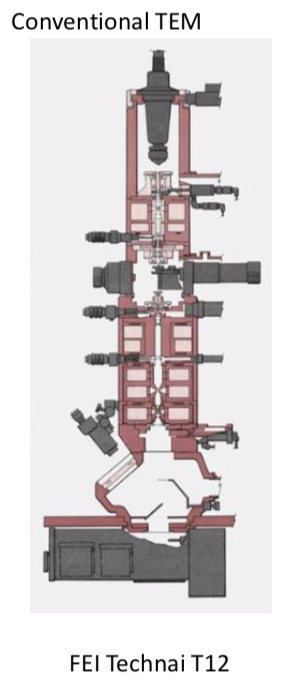
\includegraphics[width=4.22in]{images/tecnai_t12} 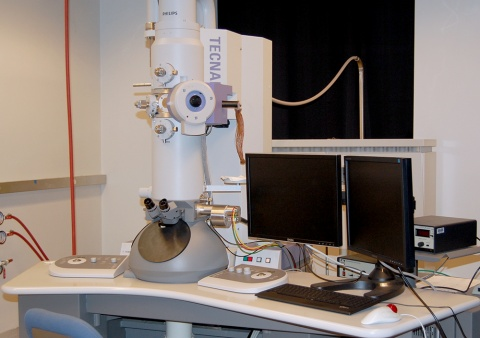
\includegraphics{images/fei-tecnai-t12.jpg}

Before you start, make sure to \textbf{1)} reserve the T12 through UMass FOM ahead of time, and \textbf{2)} sign into the T12 on UMass FOM before arriving at the Microscopy Center to initilize startup of the T12 controls.

\hypertarget{startup}{%
\chapter{Startup}\label{startup}}

During training (and being new to EM), I was instructed to first find and center the beam before loading any samples.

Take note of the IGP1. This is log(vacuum) and is never better than 6.

\begin{enumerate}
\def\labelenumi{\arabic{enumi})}
\item
  Login to computer (right monitor)
\item
  Click ``Col. Valves Closed''

  \emph{If left monitor is black. Login to T12 through UMass FOM to turn it on.}
\item
  High Tension 120V (energy of the electrons)
\item
  Turn Filament On (this takes \textasciitilde{}5min)
\item
  Find Beam

  \begin{itemize}
  \tightlist
  \item
    Use the intensity knob (L-R) to find the beam (if the intensity knobs start to beep go the other way).
  \item
    Left = under focus
  \item
    Right = Over focus
  \item
    You can also zoom out with focus if still having trouble.
  \end{itemize}
\item
  Center beam and make sure beam remains center across a range of spot sizes.

  \begin{itemize}
  \tightlist
  \item
    To move beam use ``Gun Shift'' and ``Beam Shift''. Use ``Gun Shift'' for lower spot sizes (i.e.~3, which is actully a bigger spot) and ``Beam Shift'' for higher spot sizes (i.e.~7). There is also a ``Gun Tilt'' which tilts the gun to put the most electrons in the column. I didn't really use this during my training, only the ``Gun Shift'' and ``Beam''Shift".
  \item
    You can use the multifunction x, y knobs for these
  \end{itemize}
\item
  Make the screen all beam
\end{enumerate}

You are now set to load your sample.

\hypertarget{load-sample}{%
\chapter{Load Sample}\label{load-sample}}

Once the beam is found and centered we can load the sample. We need to start by turning the T12 off so we can remove the sample holder. This process is the reverse of the ``Startup''.

\begin{enumerate}
\def\labelenumi{\arabic{enumi})}
\item
  Turn off filament
\item
  Col. Valves Closed

  \textbf{wait until filament is off}
\item
  Reset Holder (check to see x, y, and z are all close to ``0, 0, 0'')
\item
  Remove sample holder (this is a little tricky and is done in steps)

  \begin{itemize}
  \tightlist
  \item
    Pull out \textbf{gently} on sample holder until it resists \emph{and don't pull any farther}
  \item
    Rotate holder to \textasciitilde{}11 o'clock and pull all the way out.
  \end{itemize}
\end{enumerate}

\begin{figure}
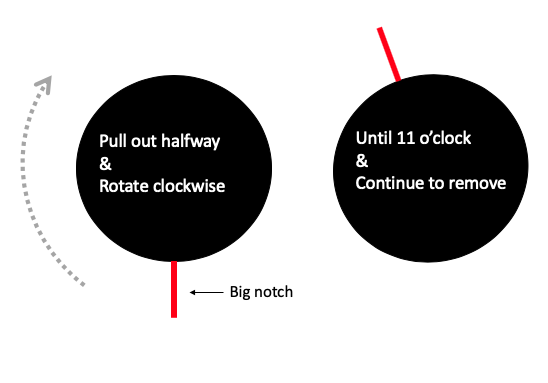
\includegraphics[width=7.61in]{images/remove_holder} \caption{Schematic of removing sample holder}\label{fig:unnamed-chunk-3}
\end{figure}

\textbf{BE CAREFUL LOADING SAMPLE HOLDER IN \& OUT. USE COMMON SENSE DON'T FORCE ANYTHING}

\begin{enumerate}
\def\labelenumi{\arabic{enumi})}
\setcounter{enumi}{4}
\tightlist
\item
  Load Sample

  \begin{itemize}
  \tightlist
  \item
    Do not ever touch sample holder below rubber o-ring
  \end{itemize}
\end{enumerate}

\begin{figure}
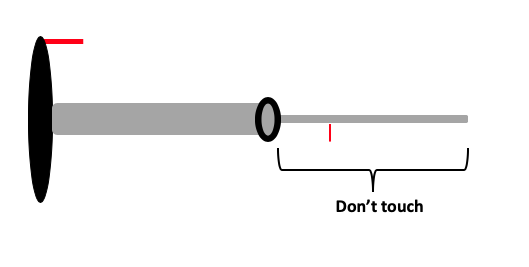
\includegraphics[width=7.35in]{images/side_view_holder} \caption{Side view of sample holder}\label{fig:unnamed-chunk-4}
\end{figure}

\begin{enumerate}
\def\labelenumi{\arabic{enumi})}
\setcounter{enumi}{5}
\tightlist
\item
  Put sample holder back into T12

  \begin{itemize}
  \tightlist
  \item
    Line up the small pin (below the o-ring) with the ``close'' on the T12. The big notch
    should be around 11 o'clock.
  \item
    Push in halfway until you feel it ``catch''. If done correctly the vacuum pump timer on the left monitor will jump down to 2 min.
  \item
    Wait the 2 minutes for the vacuum pump to turn off, rotate sample holder 60 degrees so the big notch lines up with the slot in the T12, and place in the scape. Try to do this step in one smooth quick motion. \textbf{DO NOT LET GO}. There will be some pressure from the vacuum sucking the holder in.
  \end{itemize}
\end{enumerate}

The sample is now in the scope ready to be imaged.

\hypertarget{imaging}{%
\chapter{Imaging}\label{imaging}}

This section is the most incomplete of my notes.

\begin{enumerate}
\def\labelenumi{\arabic{enumi})}
\tightlist
\item
  Find the surface

  \begin{itemize}
  \item
    The beam should already be found and aligned. Use the screen image to try and find an area of sample on the grid. Note if all you see is black you might be over a grid bar. Move around to find a new spot.
  \item
    Use the ``Eucentric focus'' to reset to standard height
  \item
    Turn on alpha-wobble
  \item
    Use the z-axis control to move the stage toward the surface.
  \item
    You will be near focus once the movement of the sample is minimal with alpha wobbler on.
  \end{itemize}
\item
  Take Pictures

  \begin{itemize}
  \item
    The MCSL Server is the Camera (on right monitor).
  \item
    To take picture:

    \begin{itemize}
    \tightlist
    \item
      Hit ``STOP''
    \item
      Select slot
    \item
      Hit the camera icon. There are two camers modes. 1) for Live mode viewing and 2) for taking static images.
    \end{itemize}
  \end{itemize}
\end{enumerate}

The files are saved to: Computer \textgreater{} Home \textgreater{} T12 \textgreater{} {[}The Day's Folder{]}

\bibliography{book.bib,packages.bib}


\end{document}
